\section{Architecture details}
\label{sec:architecture}

This section provides the particular details of the model as described in section~\ref{sec:model}. The perceptual module $f^\textit{percept}$ is a convolutional network (CNN) followed by a fully connected layer. The CNN has a first layer with 16 8x8 filters of stride 4, followed by a layer with with 32  4x4 filters of stride 2. The fully connected layer has 256 hidden units.  Each convolutional and fully-connected layer is followed by a rectifier non-linearity\footnote{This is substantially the same CNN as in~\cite{mnih2016asynchronous,mnih-dqn-2015}, the only difference is that in the pre-processing stage we retain all colour channels.}. The state space which the Manager implicitly models in formulating its goals is computed via $f^\textit{Mspace}$, which is another fully connected layer followed by a rectifier non-linearity. The dimensionality of the embedding vectors, $w$, is set as $k=16$. To encourage exploration in transition policy, at every step with a small probability $\epsilon$ we emit a random goal sampled from a uni-variate Gaussian.

The Worker's recurrent network $f^\textit{Wrnn}$ is a standard LSTM~\cite{hochreiter1997lstm}. For the Manager's recurrent network,  $f^\textit{Mrnn}$, we propose a novel  design -- the dilated LSTM, which is introduced in the next section. Both  $f^\textit{Mrnn}$ and $f^\textit{Wrnn}$ have $256$ hidden units.

\begin{figure*}[th]
\subfloat[]{ \adjustbox{trim={.1\width} {.6\height} {.7\width} {.07\height},clip}%
{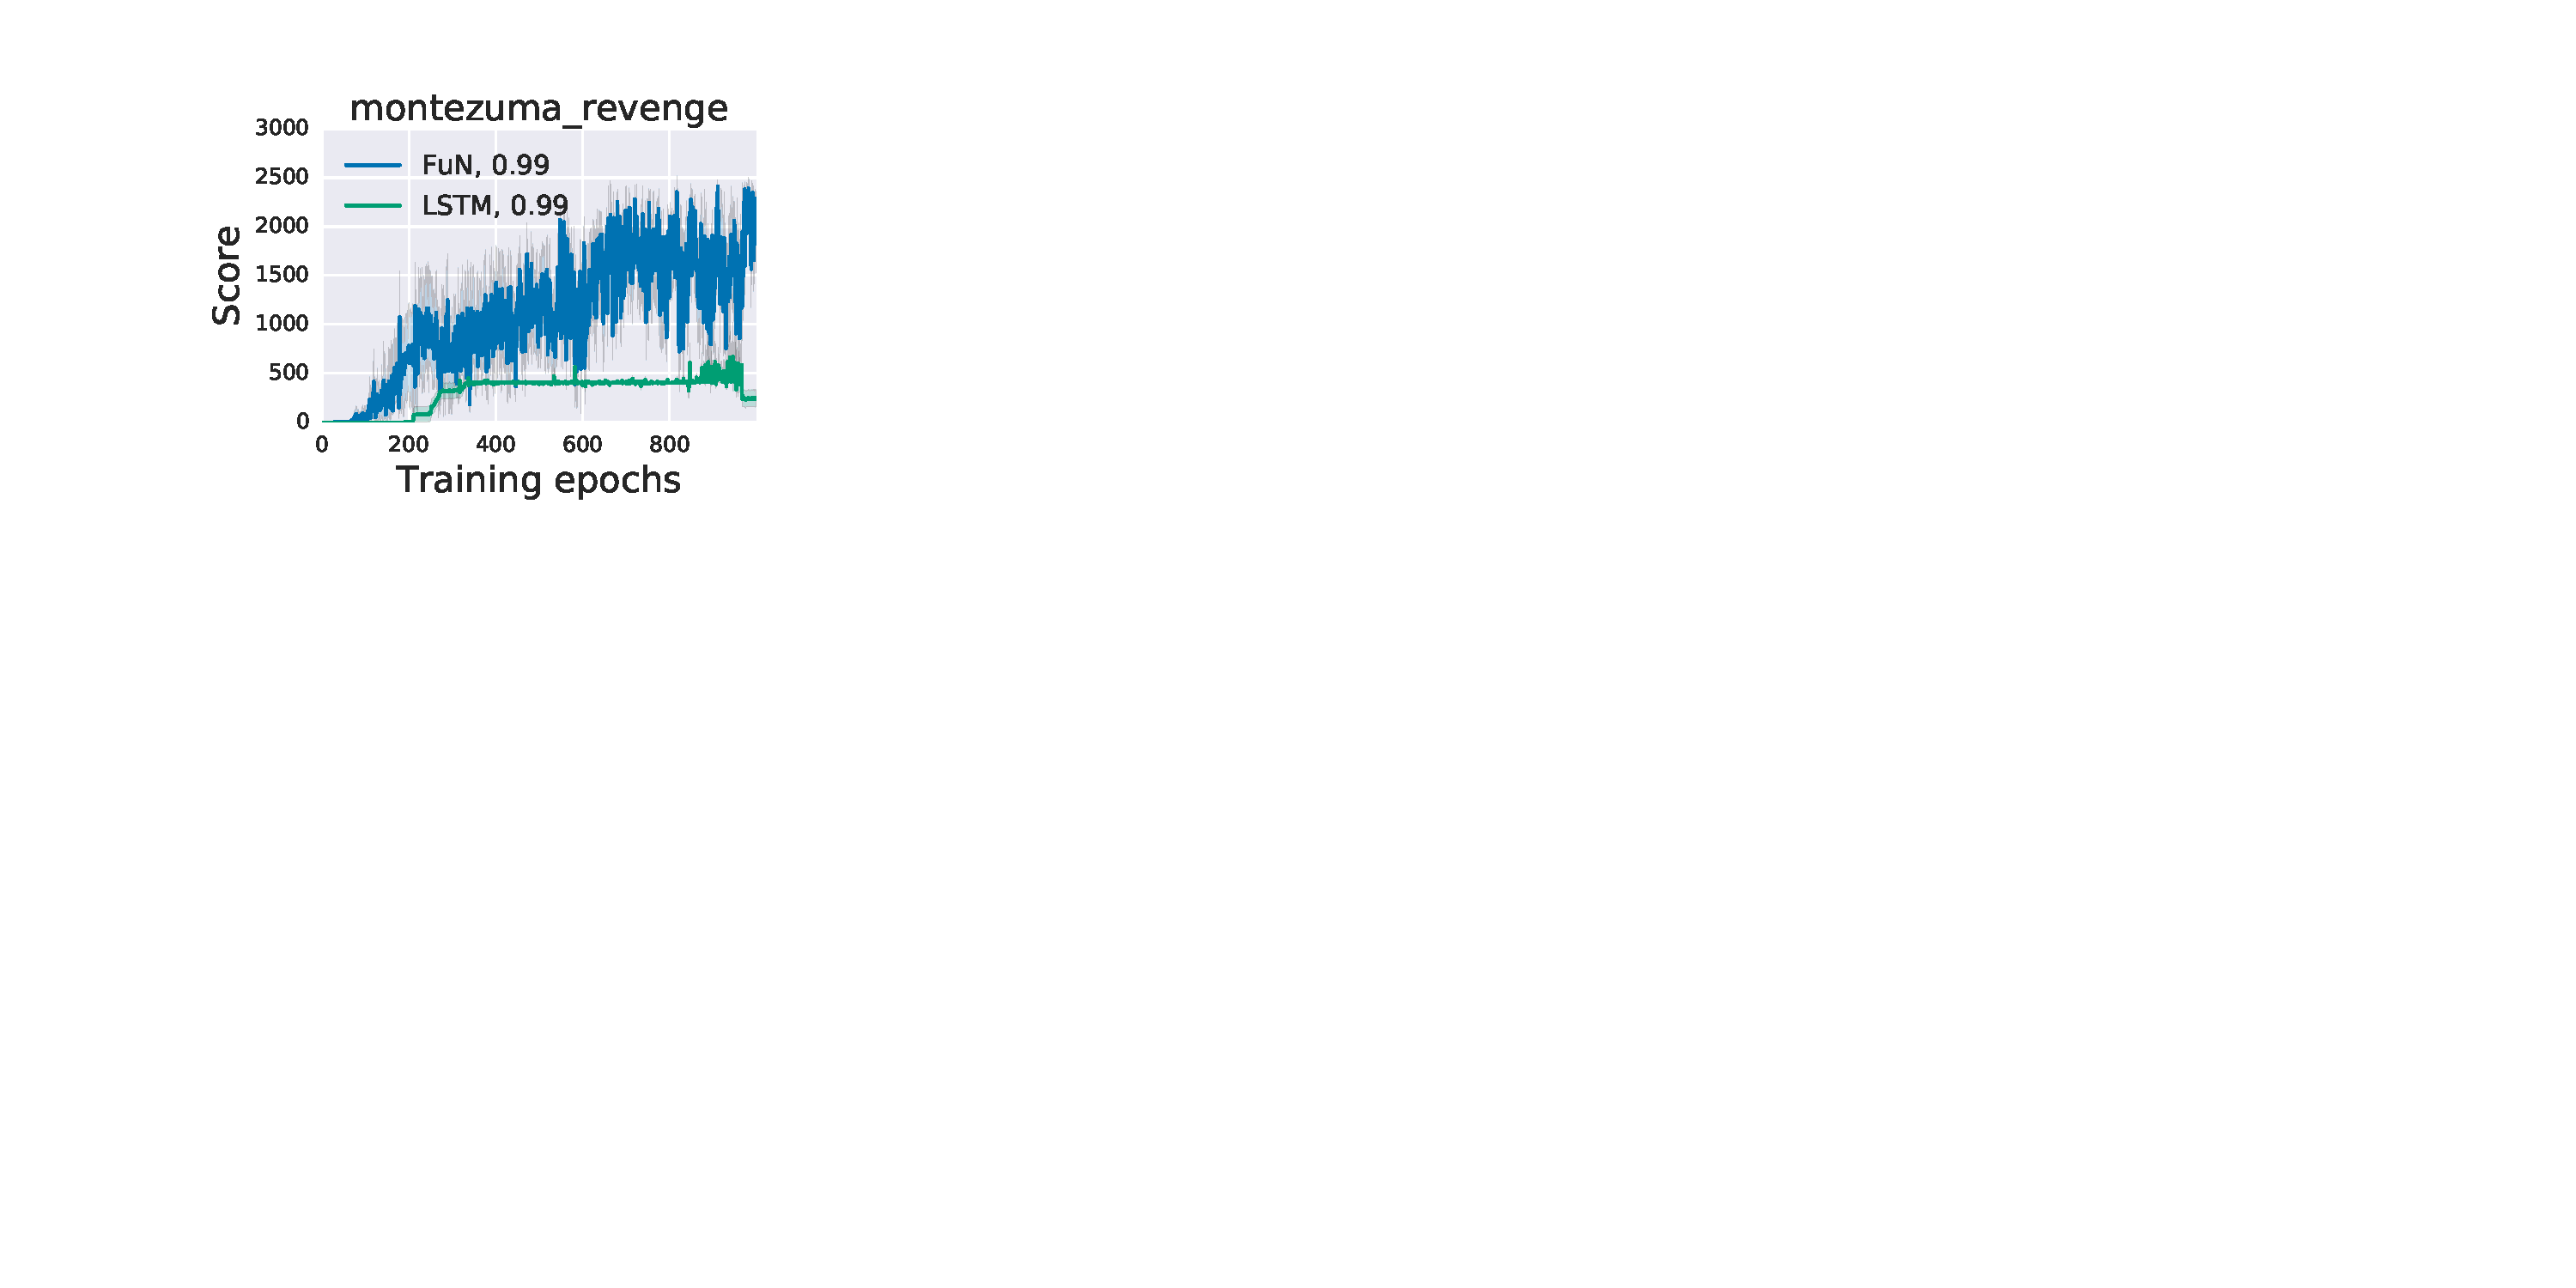
\includegraphics[scale=0.5]{./Figures/MZ_graph.pdf}}  } \hspace{25mm}
\subfloat[]{ 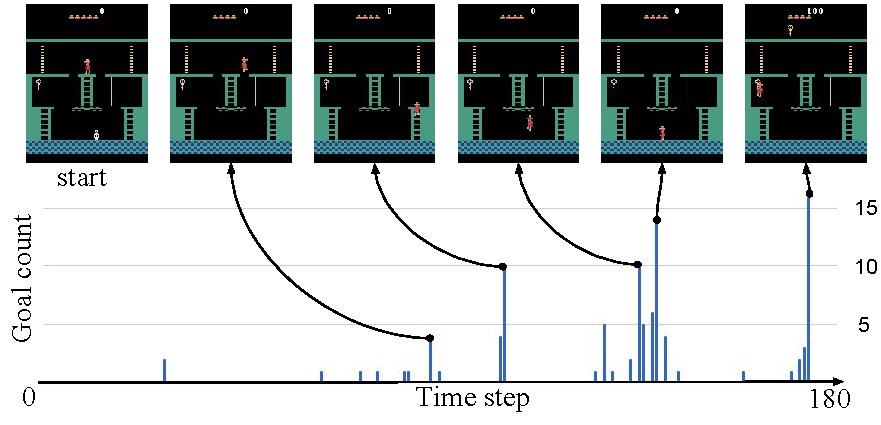
\includegraphics[scale=0.6]{./Figures/Montezuma_subgoals.pdf} }
\caption{a) Learning curve on Montezuma's Revenge b) This is a visualisation of sub-goals learnt by FuN in the first room. For each time step we compute the latent state $s_t$ and the corresponding goal $g_t$. We then find a future state for which $\cos(s_{t’} - s_t, g_t)$ is maximized. The plot corresponds to the number of past states for which a frame maximizes the goal - i.e. the taller the bar, the more frequently that state was a maximizer of the expression for some previous state. Notice that FuN has learnt a semantically meaningful sub-goals -- the tall bars in the plot (i.e. consistent goals) correspond to interpretably useful “waypoints” in Montezuma.\label{fig:Montezuma} \figskiny }
\end{figure*}

\subseckiny
\subsection{Dilated LSTM}
\subseckiny
\label{subsec:dLSTM}
We propose a novel RNN architecture for the Manager, which operates at lower temporal resolution than the data stream. We define a dilated LSTM analogously to dilated convolutional networks~\cite{yu2015dilated}. For a dilation radius $r$ let the full state of the network be $h = \{\hat{h}^i\}_{i=1}^r$, i.e. it is composed of $r$ separate groups of sub-states or `cores'. At time $t$ the network is governed by the following equations:
$\hat{h}^{t\%r}_t,g_t = \textit{LSTM}(s_t, \hat{h}^{t\%r}_{t-1}; \theta^{\textit{LSTM}})$,
where $\%$ denotes the modulo operation and allows us to indicate which group of cores is currently being updated. 
We make the parameters of the LSTM network $\theta^{\textit{LSTM}}$ explicit to stress that the same set of parameters governs the update for each of the $r$ groups within the dLSTM. 

At each time step only the corresponding part of the state is updated and the output is pooled across the previous $c$ outputs. This allows the $r$ groups of cores inside the dLSTM to preserve the memories for long periods, yet the dLSTM as a whole is still able to process and learn from every input experience, and is also able to update its output at every step. 
This idea is similar to clockwork RNNs~\cite{koutnik2014clockwork}, however there the top level ``ticks'' at a fixed, slow pace, whereas the dLSTM observes all the available training data instead. In the experiments we set $r=10$, and this was also used as the predictions horizon, $c$.